% Graphic for TeX using PGF
% Title: /home/pal/code/TSEA29/gloria/dokumentation/designspecifikation/FLOW1.dia
% Creator: Dia v0.97.2
% CreationDate: Mon Oct 13 14:12:34 2014
% For: pal
% \usepackage{tikz}
% The following commands are not supported in PSTricks at present
% We define them conditionally, so when they are implemented,
% this pgf file will use them.
\ifx\du\undefined
  \newlength{\du}
\fi
\setlength{\du}{15\unitlength}
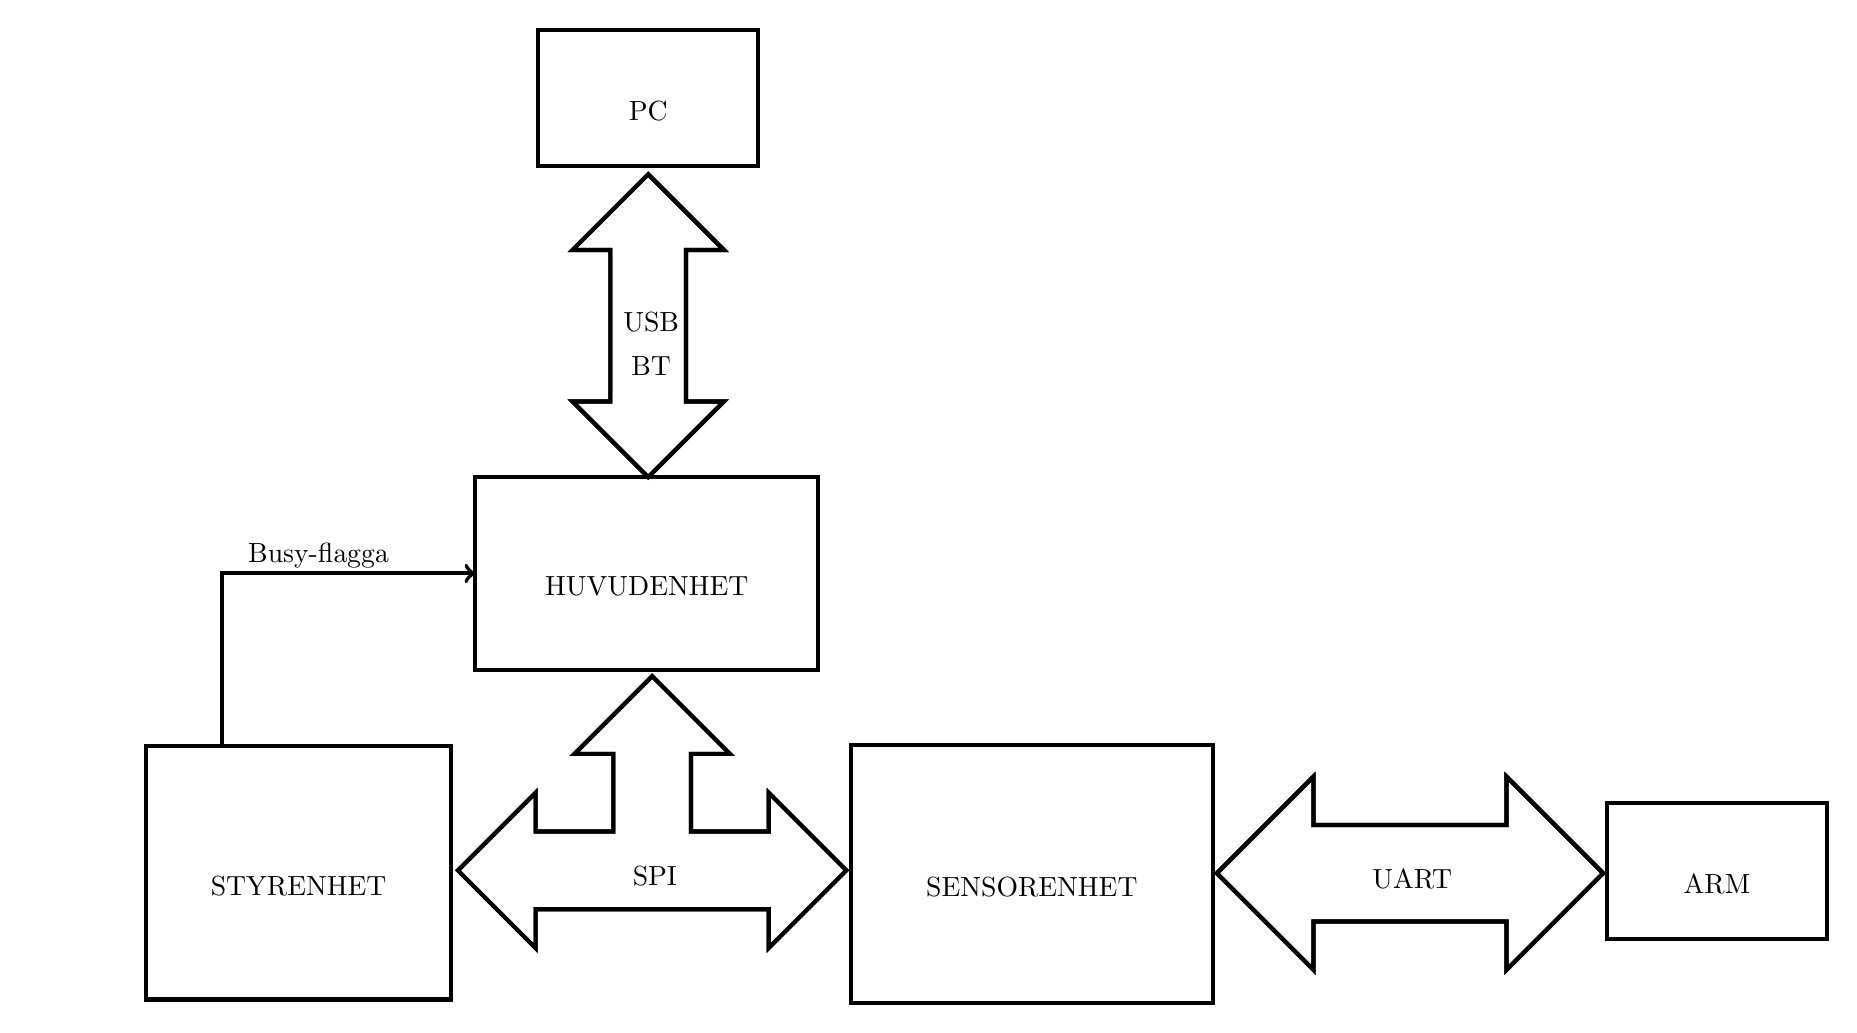
\begin{tikzpicture}
\pgftransformxscale{1.000000}
\pgftransformyscale{-1.000000}
\definecolor{dialinecolor}{rgb}{0.000000, 0.000000, 0.000000}
\pgfsetstrokecolor{dialinecolor}
\definecolor{dialinecolor}{rgb}{1.000000, 1.000000, 1.000000}
\pgfsetfillcolor{dialinecolor}
\definecolor{dialinecolor}{rgb}{1.000000, 1.000000, 1.000000}
\pgfsetfillcolor{dialinecolor}
\fill (-6.983213\du,15.055329\du)--(-6.983213\du,19.720514\du)--(1.274287\du,19.720514\du)--(1.274287\du,15.055329\du)--cycle;
\pgfsetlinewidth{0.100000\du}
\pgfsetdash{}{0pt}
\pgfsetdash{}{0pt}
\pgfsetmiterjoin
\definecolor{dialinecolor}{rgb}{0.000000, 0.000000, 0.000000}
\pgfsetstrokecolor{dialinecolor}
\draw (-6.983213\du,15.055329\du)--(-6.983213\du,19.720514\du)--(1.274287\du,19.720514\du)--(1.274287\du,15.055329\du)--cycle;
% setfont left to latex
\definecolor{dialinecolor}{rgb}{0.000000, 0.000000, 0.000000}
\pgfsetstrokecolor{dialinecolor}
\node at (-2.854463\du,17.697921\du){HUVUDENHET};
\definecolor{dialinecolor}{rgb}{1.000000, 1.000000, 1.000000}
\pgfsetfillcolor{dialinecolor}
\fill (-14.919953\du,21.553356\du)--(-14.919953\du,27.653356\du)--(-7.565446\du,27.653356\du)--(-7.565446\du,21.553356\du)--cycle;
\pgfsetlinewidth{0.100000\du}
\pgfsetdash{}{0pt}
\pgfsetdash{}{0pt}
\pgfsetmiterjoin
\definecolor{dialinecolor}{rgb}{0.000000, 0.000000, 0.000000}
\pgfsetstrokecolor{dialinecolor}
\draw (-14.919953\du,21.553356\du)--(-14.919953\du,27.653356\du)--(-7.565446\du,27.653356\du)--(-7.565446\du,21.553356\du)--cycle;
% setfont left to latex
\definecolor{dialinecolor}{rgb}{0.000000, 0.000000, 0.000000}
\pgfsetstrokecolor{dialinecolor}
\node at (-11.242700\du,24.913356\du){STYRENHET};
\definecolor{dialinecolor}{rgb}{1.000000, 1.000000, 1.000000}
\pgfsetfillcolor{dialinecolor}
\fill (2.058017\du,21.527620\du)--(2.058017\du,27.727620\du)--(10.785517\du,27.727620\du)--(10.785517\du,21.527620\du)--cycle;
\pgfsetlinewidth{0.100000\du}
\pgfsetdash{}{0pt}
\pgfsetdash{}{0pt}
\pgfsetmiterjoin
\definecolor{dialinecolor}{rgb}{0.000000, 0.000000, 0.000000}
\pgfsetstrokecolor{dialinecolor}
\draw (2.058017\du,21.527620\du)--(2.058017\du,27.727620\du)--(10.785517\du,27.727620\du)--(10.785517\du,21.527620\du)--cycle;
% setfont left to latex
\definecolor{dialinecolor}{rgb}{0.000000, 0.000000, 0.000000}
\pgfsetstrokecolor{dialinecolor}
\node at (6.421767\du,24.937620\du){SENSORENHET};
\definecolor{dialinecolor}{rgb}{1.000000, 1.000000, 1.000000}
\pgfsetfillcolor{dialinecolor}
\fill (-5.473100\du,4.291205\du)--(-5.473100\du,7.569627\du)--(-0.169808\du,7.569627\du)--(-0.169808\du,4.291205\du)--cycle;
\pgfsetlinewidth{0.100000\du}
\pgfsetdash{}{0pt}
\pgfsetdash{}{0pt}
\pgfsetmiterjoin
\definecolor{dialinecolor}{rgb}{0.000000, 0.000000, 0.000000}
\pgfsetstrokecolor{dialinecolor}
\draw (-5.473100\du,4.291205\du)--(-5.473100\du,7.569627\du)--(-0.169808\du,7.569627\du)--(-0.169808\du,4.291205\du)--cycle;
% setfont left to latex
\definecolor{dialinecolor}{rgb}{0.000000, 0.000000, 0.000000}
\pgfsetstrokecolor{dialinecolor}
\node at (-2.821454\du,6.240416\du){PC};
\pgfsetlinewidth{0.100000\du}
\pgfsetdash{}{0pt}
\pgfsetdash{}{0pt}
\pgfsetbuttcap
\pgfsetmiterjoin
\pgfsetlinewidth{0.100000\du}
\pgfsetbuttcap
\pgfsetmiterjoin
\pgfsetdash{}{0pt}
\definecolor{dialinecolor}{rgb}{1.000000, 1.000000, 1.000000}
\pgfsetfillcolor{dialinecolor}
\fill (0.082658\du,23.606553\du)--(-1.788790\du,23.606553\du)--(-1.788790\du,21.735104\du)--(-0.853066\du,21.735104\du)--(-2.724515\du,19.863655\du)--(-4.595963\du,21.735104\du)--(-3.660239\du,21.735104\du)--(-3.660239\du,23.606553\du)--(-5.531688\du,23.606553\du)--(-5.531688\du,22.670828\du)--(-7.403136\du,24.542277\du)--(-5.531688\du,26.413726\du)--(-5.531688\du,25.478001\du)--(0.082658\du,25.478001\du)--(0.082658\du,26.413726\du)--(1.954107\du,24.542277\du)--(0.082658\du,22.670828\du)--cycle;
\definecolor{dialinecolor}{rgb}{0.000000, 0.000000, 0.000000}
\pgfsetstrokecolor{dialinecolor}
\draw (0.082658\du,23.606553\du)--(-1.788790\du,23.606553\du)--(-1.788790\du,21.735104\du)--(-0.853066\du,21.735104\du)--(-2.724515\du,19.863655\du)--(-4.595963\du,21.735104\du)--(-3.660239\du,21.735104\du)--(-3.660239\du,23.606553\du)--(-5.531688\du,23.606553\du)--(-5.531688\du,22.670828\du)--(-7.403136\du,24.542277\du)--(-5.531688\du,26.413726\du)--(-5.531688\du,25.478001\du)--(0.082658\du,25.478001\du)--(0.082658\du,26.413726\du)--(1.954107\du,24.542277\du)--(0.082658\du,22.670828\du)--cycle;
\pgfsetbuttcap
\pgfsetmiterjoin
\pgfsetdash{}{0pt}
\definecolor{dialinecolor}{rgb}{0.000000, 0.000000, 0.000000}
\pgfsetstrokecolor{dialinecolor}
\draw (0.082658\du,23.606553\du)--(-1.788790\du,23.606553\du)--(-1.788790\du,21.735104\du)--(-0.853066\du,21.735104\du)--(-2.724515\du,19.863655\du)--(-4.595963\du,21.735104\du)--(-3.660239\du,21.735104\du)--(-3.660239\du,23.606553\du)--(-5.531688\du,23.606553\du)--(-5.531688\du,22.670828\du)--(-7.403136\du,24.542277\du)--(-5.531688\du,26.413726\du)--(-5.531688\du,25.478001\du)--(0.082658\du,25.478001\du)--(0.082658\du,26.413726\du)--(1.954107\du,24.542277\du)--(0.082658\du,22.670828\du)--cycle;
% setfont left to latex
\definecolor{dialinecolor}{rgb}{0.000000, 0.000000, 0.000000}
\pgfsetstrokecolor{dialinecolor}
\node[anchor=west] at (-2.809581\du,23.507309\du){};
% setfont left to latex
\definecolor{dialinecolor}{rgb}{0.000000, 0.000000, 0.000000}
\pgfsetstrokecolor{dialinecolor}
\node[anchor=west] at (-3.464823\du,24.689659\du){SPI};
% setfont left to latex
\definecolor{dialinecolor}{rgb}{0.000000, 0.000000, 0.000000}
\pgfsetstrokecolor{dialinecolor}
\node[anchor=west] at (-17.819091\du,21.507679\du){};
\pgfsetlinewidth{0.100000\du}
\pgfsetdash{}{0pt}
\pgfsetdash{}{0pt}
\pgfsetbuttcap
\pgfsetmiterjoin
\pgfsetlinewidth{0.100000\du}
\pgfsetbuttcap
\pgfsetmiterjoin
\pgfsetdash{}{0pt}
\definecolor{dialinecolor}{rgb}{1.000000, 1.000000, 1.000000}
\pgfsetfillcolor{dialinecolor}
\fill (-3.732377\du,13.245589\du)--(-3.732377\du,9.598291\du)--(-4.644202\du,9.598291\du)--(-2.820553\du,7.774642\du)--(-0.996904\du,9.598291\du)--(-1.908728\du,9.598291\du)--(-1.908728\du,13.245589\du)--(-0.996904\du,13.245589\du)--(-2.820553\du,15.069238\du)--(-4.644202\du,13.245589\du)--cycle;
\definecolor{dialinecolor}{rgb}{0.000000, 0.000000, 0.000000}
\pgfsetstrokecolor{dialinecolor}
\draw (-3.732377\du,13.245589\du)--(-3.732377\du,9.598291\du)--(-4.644202\du,9.598291\du)--(-2.820553\du,7.774642\du)--(-0.996904\du,9.598291\du)--(-1.908728\du,9.598291\du)--(-1.908728\du,13.245589\du)--(-0.996904\du,13.245589\du)--(-2.820553\du,15.069238\du)--(-4.644202\du,13.245589\du)--cycle;
\pgfsetbuttcap
\pgfsetmiterjoin
\pgfsetdash{}{0pt}
\definecolor{dialinecolor}{rgb}{0.000000, 0.000000, 0.000000}
\pgfsetstrokecolor{dialinecolor}
\draw (-3.732377\du,13.245589\du)--(-3.732377\du,9.598291\du)--(-4.644202\du,9.598291\du)--(-2.820553\du,7.774642\du)--(-0.996904\du,9.598291\du)--(-1.908728\du,9.598291\du)--(-1.908728\du,13.245589\du)--(-0.996904\du,13.245589\du)--(-2.820553\du,15.069238\du)--(-4.644202\du,13.245589\du)--cycle;
% setfont left to latex
\definecolor{dialinecolor}{rgb}{0.000000, 0.000000, 0.000000}
\pgfsetstrokecolor{dialinecolor}
\node at (-2.748567\du,11.325958\du){USB};
% setfont left to latex
\definecolor{dialinecolor}{rgb}{0.000000, 0.000000, 0.000000}
\pgfsetstrokecolor{dialinecolor}
\node at (-2.748567\du,12.384292\du){BT};
\pgfsetlinewidth{0.100000\du}
\pgfsetdash{}{0pt}
\pgfsetdash{}{0pt}
\pgfsetbuttcap
\pgfsetmiterjoin
\pgfsetlinewidth{0.100000\du}
\pgfsetbuttcap
\pgfsetmiterjoin
\pgfsetdash{}{0pt}
\definecolor{dialinecolor}{rgb}{1.000000, 1.000000, 1.000000}
\pgfsetfillcolor{dialinecolor}
\fill (17.857003\du,23.448431\du)--(13.205264\du,23.448431\du)--(13.205264\du,22.285496\du)--(10.879394\du,24.611366\du)--(13.205264\du,26.937236\du)--(13.205264\du,25.774301\du)--(17.857003\du,25.774301\du)--(17.857003\du,26.937236\du)--(20.182873\du,24.611366\du)--(17.857003\du,22.285496\du)--cycle;
\definecolor{dialinecolor}{rgb}{0.000000, 0.000000, 0.000000}
\pgfsetstrokecolor{dialinecolor}
\draw (17.857003\du,23.448431\du)--(13.205264\du,23.448431\du)--(13.205264\du,22.285496\du)--(10.879394\du,24.611366\du)--(13.205264\du,26.937236\du)--(13.205264\du,25.774301\du)--(17.857003\du,25.774301\du)--(17.857003\du,26.937236\du)--(20.182873\du,24.611366\du)--(17.857003\du,22.285496\du)--cycle;
\pgfsetbuttcap
\pgfsetmiterjoin
\pgfsetdash{}{0pt}
\definecolor{dialinecolor}{rgb}{0.000000, 0.000000, 0.000000}
\pgfsetstrokecolor{dialinecolor}
\draw (17.857003\du,23.448431\du)--(13.205264\du,23.448431\du)--(13.205264\du,22.285496\du)--(10.879394\du,24.611366\du)--(13.205264\du,26.937236\du)--(13.205264\du,25.774301\du)--(17.857003\du,25.774301\du)--(17.857003\du,26.937236\du)--(20.182873\du,24.611366\du)--(17.857003\du,22.285496\du)--cycle;
\definecolor{dialinecolor}{rgb}{1.000000, 1.000000, 1.000000}
\pgfsetfillcolor{dialinecolor}
\fill (20.273254\du,22.918859\du)--(20.273254\du,26.197281\du)--(25.576545\du,26.197281\du)--(25.576545\du,22.918859\du)--cycle;
\pgfsetlinewidth{0.100000\du}
\pgfsetdash{}{0pt}
\pgfsetdash{}{0pt}
\pgfsetmiterjoin
\definecolor{dialinecolor}{rgb}{0.000000, 0.000000, 0.000000}
\pgfsetstrokecolor{dialinecolor}
\draw (20.273254\du,22.918859\du)--(20.273254\du,26.197281\du)--(25.576545\du,26.197281\du)--(25.576545\du,22.918859\du)--cycle;
% setfont left to latex
\definecolor{dialinecolor}{rgb}{0.000000, 0.000000, 0.000000}
\pgfsetstrokecolor{dialinecolor}
\node at (22.924900\du,24.868070\du){ARM};
% setfont left to latex
\definecolor{dialinecolor}{rgb}{0.000000, 0.000000, 0.000000}
\pgfsetstrokecolor{dialinecolor}
\node[anchor=west] at (14.354268\du,24.742692\du){UART};
\pgfsetlinewidth{0.100000\du}
\pgfsetbuttcap
\pgfsetdash{}{0pt}
{
\definecolor{dialinecolor}{rgb}{0.000000, 0.000000, 0.000000}
\pgfsetfillcolor{dialinecolor}
% was here!!!
\pgfsetarrowsend{to}
\definecolor{dialinecolor}{rgb}{0.000000, 0.000000, 0.000000}
\pgfsetstrokecolor{dialinecolor}
\draw (-13.081326\du,21.553356\du)--(-13.081326\du,17.387921\du)--(-6.983213\du,17.387921\du);
}
% setfont left to latex
% setfont left to latex
\definecolor{dialinecolor}{rgb}{0.000000, 0.000000, 0.000000}
\pgfsetstrokecolor{dialinecolor}
\node[anchor=west] at (-12.727822\du,16.964518\du){Busy-flagga};
\end{tikzpicture}
